{
\newcommand{\lbfont}{\small}
\def\ysb{-.15} % bottom of rigid body 
\def\ysa{-2}   % top of rigid body 
\def\ya{0} % bottom of fluid domain 
\def\yb{2} % top of fluid domain
\def\xL{5}
% ---------------------- chirp function -----------
\newcommand{\plotChirp}[1]{
\draw[draw=blue,line width=2pt] 
      plot[samples=500, domain=0.:10.2] ( {\x} , {2*sin(60*\x + #1*60*\x*\x)} );
}
%
% ---------------------------------------
%
\begin{figure}[hbt]
\newcommand{\textFont}{\normalss}
\begin{center}
  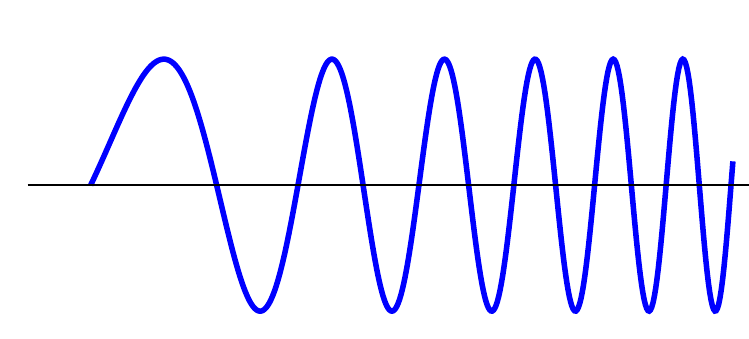
\begin{tikzpicture}[scale=.8]
  %
  \useasboundingbox (-1,0) rectangle (10,4.5);  % set the bounding box (so we have less surrounding white space)
  %
  \begin{scope}[yshift=2cm]
    \plotChirp{.25}
    \draw[->,thick,black] (-1,0) -- (11,0) node [anchor=north] {$t$}; 
  \end{scope}
%-   %
% grid:
%  \draw[step=1cm,gray] (-1,0) grid (10,4.);
  %
  \end{tikzpicture}
\end{center}
\caption{Chirp function, $\sin( \phi(t))$: the frequency increases linearly and the wavelength decreases linearly over time.}
\label{fig:chirpFunction}
\end{figure}
}
